%!TEX ROOT=sample-thesis.tex
%!TEX PROGRAM=xelatex

\chapter{Literature Review}

This chapter reviews visualization literature to outline the state of the art, taxonomy, and emerging trends of visual analytics designs and applications. A thematic taxonomy of visual analytic designs and applications was devised to guide deriving the state of the art. The taxonomy classifies visual analytics studies according to applied domains, design features, information-seeking tasks, data properties, data sources, and visualization techniques. Furthermore, summarization of the design challenges and solutions for visual analytics were highlighted. Several design challenges in reported visual analytics including visual usability and information appertains are identified. In addition, a summarization of visual analytics for MOOC and case scenarios for this study is presented. Subsequently, this chapter explores the visualization design space of visual analytics designs and applications for MOOC data. A visualization design space of visual analytics for MOOC data is elicited based on the systematic review. The design space is then explored to identify and highlight the gaps or pitfalls in the current design guideline.
\\[\baselineskip]\indent
The remainder of this chapter is as follows. Section 2.1 introduces the underlying principles and definitions in the field of visualization. Section 2.2 then discusses the state of the art of visual analytics designs and applications. In Section 2.3, a taxonomy of visual analytics designs and applications and their characterization are introduced. Section 2.4 then highlights identified design challenges, while recommendations for these challenges are presented in Section 2.5. In Section 2.6, the relations between design challenges with the case of visual analytics for MOOC data are articulated. Section 2.7 then introduces the underlying principles of visualization design space, followed by Section 2.8 that presents a systematic analysis of MOOC visualization design. Finally, the chapter is concluded in Section 2.9.


\section{Foundation and Theories of Visualization and Visual Analytics}
This section presents the comprehensive analysis results of potential research gaps highlighted from the literature review. Furthermore, potential research gaps based on the relation with the motivation of this study are discussed. Moreover, a prime research gap is selected and discussed as the central motivation of this study. Subsequently, the justifications on the importance of dealing with the selected research gap were presented.

\subsection{Information Visualization and Visual Analytics}
Visualization is the representation of an object, situation, or set of information in the form of visual such as chart or graph \parencite{Oxford2020}. Visualization is also defined as the formation of human cognitive mental visual images, or the activity of interpreting in visual terms or of realizing it into visible form \parencite{Merriam2020,Owen1999}. This definition is then extended as “a tool or method for interpreting image data fed into a computer and for generating images from complex multi-dimensional data sets” \parencite{Owen1999}. Visualization techniques have been traditionally categorized into two major areas:
\begin{itemize}
\item Scientific visualization – visualization that involves scientific data with an inherent physical component.
\item Information visualization – visualization that involves abstract, nonspatial data.
\end{itemize}

\indent Information visualization is also known as the study of visual representations of abstract information to amplify the human cognition. When human is engaged through interaction with visual object (what they see with their eyes), there is an internal mental construction of information processing in their mind. Generally, visualization is a cognitive activity that is facilitated by external visual representations where human build an internal mental representation of it. Visual representations such as pictorials, graphs, and symbols help us to understand the external data thus producing better information understanding \parencite{Mazza2009}. The visualization process starts with refining or filtering the raw data, which then classified into data tables. The data then undergo visual structuring and then presented in the appropriate views \parencite{Card1999}. The whole process was shown in the Figure \ref{visual}. \\

\begin{figure}[hbt!]
\centering
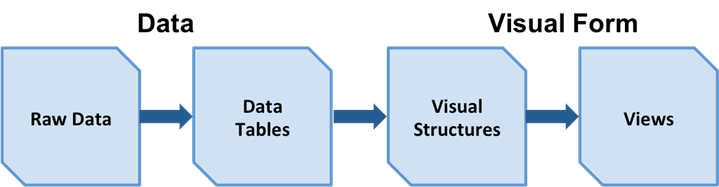
\includegraphics[scale=1]{Fig2.1}
\caption[Information visualization model]{Information visualization model\\\source{Card (1999)}}
\label{visual}
\end{figure}

\indent Visual analytics is a science of analytical reasoning facilitated by interactive visual interfaces. This thesis assert “interaction” as the key role of visual analytics as it facilitates interactivity between automated data analysis, visualization, and human user. Visual analytics enables human user to gain insights into solving complex problems by leveraging domain knowledge and intuition input with computer processing prowess. The exponential growth in data analytics utilization and visually driven data across many domains contributes to the rising need for effective visual analytics.
